\documentclass[12pt,a4paper]{report}

% Packages

\usepackage[utf8]{inputenc}
\usepackage[italian]{babel}
\usepackage{lipsum}
\usepackage{csquotes}
\usepackage{graphicx}
\usepackage{tabulary}
\usepackage{rotating}
\usepackage{float}
\usepackage{setspace}
\usepackage[acronym]{glossaries}
\usepackage[backend=bibtex,
style=numeric,
defernumbers=true,
%style=reading,
%style=alphabetic,
bibencoding=ascii,
sorting=ynt
]{biblatex}
\usepackage{geometry}
\geometry
{
    a4paper,
    total={170mm,257mm},
    left=35mm,
    right=35mm,
    top=40mm,
    bottom=40mm
}

\restylefloat{table}

% Interlinea 1,5
\onehalfspacing

% Crea il glossario
\makeglossaries
% Acronym definitions

\newacronym{api}   {API}      {Application Programming interface}
\newacronym{css}    {CSS}       {Cascading Style Sheets}
\newacronym{dom}    {DOM}       {Document Object Model}
\newacronym{gui}    {GUI}       {Graphical User Interface}
\newacronym{el}     {EL}        {Electron}
\newacronym{html}   {HTML}      {Hypertext Markup Language}
\newacronym{ipc}   {IPC}      {Inter-Process Communication}
\newacronym{json}   {JSON}      {JavaScript Object Notation}
\newacronym{uml}   {UML}      {Unified Modeling Language}

% Imposta il percorso delle immagini
\graphicspath{ {Immagini/} }

% Crea la bibliografia
\addbibresource{biblio}

\begin{document}

    \begin{titlepage}
    
    	\centering
    	{\scshape\LARGE Università degli studi di Camerino \par}
    	
    	\vspace{0.5cm}
    	{\scshape\Large Scuola di Scienze e Tecnologie\par}
    	
    	\vspace{0.5cm}
    	{\scshape Corso di Laurea in Informatica (L-31)\par}
    	
    	\vspace{1cm}
    	
\includegraphics[width=4cm]{unicam-scudo.png}\par\vspace{1cm}
    	{\huge\bfseries Progettazione e sviluppo di un applicazione desktop per l'analisi di bilancio di un'azienda\par}
    	\vspace{2cm}
    	
    	{Laureando \hfill Relatrice \par}
    	{\bfseries \large Danilo Paoletti \hfill Dr.ssa Barbara Re \par}
    	{\small Matricola 085353 \hfill}
    
    	\vfill
    	
    	% Bottom of the page
    	{\large Anno accademico 2017-2018\par}
    	
    \end{titlepage}
    
    % White page
    \thispagestyle{empty}
    \clearpage\null\newpage
    
    % Inizia la numerazione Romana delle pagine
    \setcounter{page}{3}
    \pagenumbering{Roman}
    	
    \tableofcontents
    
    % White page
    \clearpage\null\newpage
    
    % Inizia la numerazione Araba delle pagine
    \pagenumbering{arabic}
    
    % Introduzione
    %\chapter{Introduzione}
\chapter*{Introduzione}
\addcontentsline{toc}{chapter}{Introduzione}
\markboth{INTRODUCTION}{}

L'analisi di bilancio è una delle procedure attraverso cui vegono determinati i fattori che determinano i guadagni, le risorse attraverso cui l'azienda ripaga i debiti e il grado di indebitamento.
In questa tesi verrà mostrato il software da me realizzato per il processo di analisi di bilancio attraverso la riclassificazione dello Stato Patrimoniale, del Conto Economico e del forecast per indici di previsioni.\\
Inizialmente verrà descritto il contesto economico dell'analisi di bilancio, successivamente verranno trattate la fase di analisi e progettazione che ha preceduto la realizzazione del software, descrivendo attraverso diagramma \Gls{uml} \cite{uml} i vari requisiti, vincoli e funzionalità del prodotto. \\
Successivamente saranno descritte le tecnologie utilizzate e si entrerà nel merito della realizzazione di tutte le funzionalità richieste. \\
In conclusione si farà riferimento ad eventuali sviluppi futuri che potrebbero essere implementati nel software realizzato.
    
    % White page
    \clearpage\null\newpage
    
    % Bilancio di un'azienda
    % 2

\chapter{Bilancio di un'azienda}

L’analisi di bilancio, è uno strumento tecnico, che permette di studiare i risultati d’esercizio derivanti dalle attività aziendali, focalizzando l’attenzione su:
\begin{itemize}
 \item situazione economica: condizioni che determinano la produttività dell’azienda e costituisce la capacità di determinare utili d’esercizio;
 \item situazione finanziaria: condizioni che determinano la capacità di far fronte ai debiti a breve scadenza e all’accesso a prestiti di finanziamento;
 \item situazione patrimoniale: condizioni che determinano il rapporto tra le immobilizzazioni e i debiti verso terzi.
\end{itemize}
In altre parole, con lo strumento dell’analisi di bilancio, si cerca di individuare nelle diverse aree (economica, finanziaria e patrimoniale) i primi spunti di riflessione per l’analisi della gestione.

Il bilancio di un'azienda, nella sua forma più semplice, è formato da due documenti: lo \textbf{Stato Patrimoniale},che rappresenta in modo sintetico la composizione qualitativa e quantitativa del patrimonio della società al giorno della chiusura dell’esercizio, e il \textbf{Conto Economico}, che espone il risultato economico dell’esercizio attraverso la rappresentazione dei costi e degli oneri sostenuti, nonché dei ricavi e degli altri proventi conseguiti nell’esercizio;.


% 2.1

\section{Stato Patrimoniale}

Lo Stato Patrimoniale, definito dall'art. 2424 del Codice Civile, rappresenta la situazione patrimoniale ad una certa data di un'impresa ed è suddiviso in due sezioni contrapposte chiamate Attività e Passività.

In particolare, le attività sono distinte secondo criteri di realizzabilità ed esigibilità, in :
\begin{itemize}
 \item crediti verso soci per versamenti ancora dovuti, con separata indicazione della parte già richiamata;
 \item immobilizzazioni: rappresentano gli investimenti destinati per un periodo superiore a 12 mesi, a trasformarsi in denaro. Sono iscritte al netto dei fondi di ammortamento;
 \item attivo circolante: rappresentano gli investimenti destinati per un periodo inferiore a 12 mesi, a trasformarsi in denaro. Iscritto al netto di eventuali fondi di svalutazione;
 \item ratei e riscontri;
\end{itemize}

Le passività, nell’analisi di bilancio, vengono distinte secondo le scadenze di pagamento in:
\begin{itemize}
 \item patrimonio netto;
 \item fondi per rischi e oneri;
 \item trattamento di fine rapporto di lavoro subordinato;
 \item debiti;
 \item ratei e riscontri;
\end{itemize}

Si possono individuare due criteri di riclassificazione dello stato patrimoniale per acquisire migliori informazioni sulle dinamiche aziendali: il criterio funzionale e quello finanziario.

% 2.1.1

\subsection{Riclassificazione Funzionale (Operativo)}

Secondo il criterio funzionale invece le attività (impieghi) e le passività (fonti) sono riclassificate in base all’area gestionale di appartenenza: area caratteristica/operativa (nella quale ricomprendere se marginale anche quella accessoria), comprendente tutti i valori attinenti il core business; area finanziaria, comprendente tutti i valori relativi alla negoziazione di liquidità.\\
Gli impieghi sono pertanto suddivisi in:
\begin{itemize}
\item attività operative: assets materiali e immateriali, crediti operativi, rimanenze, ratei e risconti;
\item attività finanziarie: investimenti finanziari (a breve e a medio-lungo), crediti finanziari e disponibilità liquide.
\end{itemize}

Le fonti sono invece suddivise in:
\begin{itemize}
\item patrimonio netto: grandezza non riconducibile né all’area operativa né a quella finanziaria;
\item passività operative: fondi rischi ed oneri, debiti operativi e ratei e risconti;
\item passività finanziarie: ovvero i debiti finanziari a prescindere dalla scadenza.
\end{itemize}

Lo stato patrimoniale classificato secondo la logica funzionale mira a verificare l’equilibrio fra investimenti e fonti di finanziamento, e quindi di ausilio a sviluppare l’analisi della solidità

% 2.1.2

\subsection{Riclassificazione Finanziario}

Con il criterio finanziario le attività (impieghi) sono classificate e raggruppate secondo il loro grado di liquidabilità, ovvero in funzione della loro capacità di trasformarsi in liquidità in tempi più o meno rapidi, mentre le passività (fonti) in base alla loro durata temporale, ovvero in base alla loro velocità di estinzione.

L’arco temporale preso a riferimento con termine congruo per circoscrivere il breve dal medio-lungo termine corrisponde a 12 mesi.

Gli impieghi sono pertanto suddivisi, in funzione alla loro effettiva possibilità di trasformarsi in liquidità, in:
\begin{itemize}
 \item attività correnti, atte ad essere liquidate in un arco temporale inferiore a 12 mesi, ovvero assets destinati alla vendita entro 12 mesi, attività finanziarie detenute a scopo di negoziazione, crediti in scadenza entro 12 mesi, rimanenze (per la parte che presenta un tasso di rotazione inferiore a 12 mesi), liquidità, ratei e risconti;
 \item attività non correnti, destinate a rimanere vincolate nel medio-lungo periodo, ovvero assets materiali, immateriali e finanziarie (eccetto quelle destinate alla vendita nel breve termine), crediti con scadenza oltre il 12 mesi, rimanenze (per la parte che presenta un tasso di rotazione inferiore a 12 mesi).
\end{itemize}

Le fonti sono invece suddivise in:
\begin{itemize}
 \item patrimonio netto, grandezza vincolata e quindi fonte di lungo periodo;
 \item passività correnti, destinate al rimborso entro i 12 mesi, ossia: debiti a breve (comprese le rate a breve di finanziamenti a medio-lungo termine), ratei e risconti passivi, fondi rischi ed oneri (per la parte che avrà manifestazione finanziaria nel breve periodo);
 \item passività non correnti, con scadenza superiore a 12 mesi, ossia: debiti a medio-lungo, risconti passivi pluriennali, fondi rischi ed oneri (per la parte che avrà manifestazione finanziaria oltre 12 mesi).
\end{itemize}

Lo stato patrimoniale classificato secondo la logica finanziaria permette di verificare la capacità dell’azienda di far fronte ai propri impegni di breve periodo con impieghi di egual durata (capitale circolante), ed è pertanto propedeutico all’analisi della liquidità;
\\
\\
\\

% 2.2

\section{Conto Economico}

Il Conto Economico, definito dall'art. 2425 del Codice Civile, è l'elenco, ordinato per categorie, dei costi e dei ricavi di competenza dell'esercizio, ossia di competenza di quel lasso di tempo intercorrente tra la data di riferimento del bilancio attuale e quella del bilancio precedente.

Si intendono ricavi le vendite dei propri beni, gli interessi attivi o i fitti attivi. 
Sono, invece, esempi di costi gli acquisti, le utenze, le spese del personale, i fitti passivi le imposte e le tasse. 

In tale contesto è bene far presente che l'Iva, ancorché un'imposta, non rappresenta un costo per la società. \\
Si tratta, infatti, di un debito o un credito che l'azienda ha nei confronti dell'Erario nel momento in cui compie una vendita o un acquisto e, per questo motivo, trova allocazione nel passivo o nell'attivo dello Stato Patrimoniale.

Esso ha una struttura a forma scalare e una classificazione dei costi per natura (invece che per destinazione). È formato da quattro sezioni (individuate con le prime lettere dell'alfabeto), più alcune voci che illustrano il risultato d'esercizio, ante e dopo le imposte.

Sezioni che compongono il conto economico:
\begin{itemize}
 \item valore della produzione;
 \item costi della produzione;
 \item proventi ed oneri finanziari;
 \item rettifiche di valore di attività e passività finanziarie.
\end{itemize}

Il Conto Economico può assumere diverse forme e configurazioni. Le riclassificazioni più utilizzate, per l’analisi di bilancio sono:
\begin{itemize}
\item il conto economico a margine di contribuzione, che si basa sulla suddivisione dei costi operativi tra costi fissi e costi variabili;
\item il conto economico a costo del venduto, che si basa sulla suddivisione dei costi operativi tra costi diretti e costi indiretti;
\item il conto economico a valore aggiunto, che si basa sulla suddivisione dei costi operativi tra costi relativi alle risorse esterne e costi relativi alle risorse interne.
 \end{itemize}

Nel software è stata presa in considerazione solo la riclassificazione a valore aggiunto.

% 2.2.2

\subsection{Riclassificazione al Valore Aggiunto}

Il valore aggiunto, quale differenza tra ricavi operativi e costi operativi sostenuti per l’acquisto di risorse esterne, esprime la capacità dell’azienda di creare ricchezza per remunerare i fattori produttivi e i diversi portatori di interesse.

In particolare tale margine deve essere in grado di remunerare:
\begin{itemize}
\item il personale - costo del personale;
\item gli investimenti - ammortamenti e svalutazioni;
\item i finanziatori esterni - componenti finanziarie;
\item gli eventi straordinati - componenti straordinarie;
\item l’Amministrazione finanziaria - imposte.
\end{itemize}

Deve infine garantire un’adeguata remunerazione, tramite la distribuzione del risultato d’esercizio, ai soci e permettere con l’utile residuo non distribuito un adeguato autofinanziamento.


% 2.3

\section{Forecast}

Il Forecast è un prospetto simile a un normale bilancio. A differenza di quest’ultimo, che registra valori a consuntivo, il Forecast è una tabella che contiene valori di natura previsionale. Nello specifico, dà una previsione che guarda avanti di qualche mese.

L’impostazione e lo scopo del Forecast sono simili a quelli del budget. Cambia però il periodo di analisi. Infatti, mentre il budget è una previsione fatta sull’anno successivo, il Forecast è una previsione sull’anno in corso.


    
    % White page
    \clearpage\null\newpage
    
    % Analisi del progetto
    % 3

\chapter{Analisi e progettazione}

% 3.1

\section{Descrizione del problema}

Si vuole realizzare un'applicazione desktop per l'analisi di bilancio di un'azienda per l'ordine dei commercialisti della provincia di Ancona.
L'applicazione deve funzionare in tutti i vari tipi di sistema operativo, perciò il software deve essere cross-platform.
Per poter realizzare un prodotto che sia cross-platform, ossia implementato per più piattaforme di elaborazione, la scelta delle tecnologie da utilizzare è stata fondamentale.
Quando si vuole sviluppare un'applicazione desktop la prima cosa a cui si pensa è per quale sistema operativo svilupparla, quale linguaggio usare ed opzionalmente a quale base dati si ha bisogno di connettersi.
Il mondo dell'informatica intanto si sta evolvendo verso l'utilizzo di applicazioni web per la loro semplicità di distribuzione e aggiornamento, la compatibilità con ogni sistema operativo e la superfluità di un'installazione, allora perchè non sfruttare questa tecnologia?
Per questo la scelta è ricaduta su un compromesso valido, Electron.
Definita dallo slogan "Build cross platform desktop apps with Javascript, HTML, and CSS", Electron è una libreria open source sviluppata dal team di GitHub che permette di sviluppare un’applicazione desktop utilizzando le stesse tecnologie di un sito web, unendo la potenza del browser Chromium, la flessibilità di Node.js e il più grande ecosistema di librerie open source al mondo: npm. In aggiunta a tutto questo la possibilità di pacchettizzare l’applicazione per Mac, Windows, e Linux con lo stesso risultato in termini di grafica e funzionalità.

L'applicazione realizzata, nello specifico, dovrà permettere all'utente che la utilizza l'inserimento in input dei dati relativi all'Anagrafica, all'Analisi Qualitativa, dello Stato Patrimoniale e del Conto Economico di un'azienda.
Nella fase di inserimento dei valori dello Stato Patrimoniale e del Conto Economico, il sistema calcola le varie riclassificazioni dello Stato Patrimoniale (Funzionale, Finanziario o entrambi, a seconda della scelta da parte dell'utente) e del Conto Economico (al Valore Aggiunto).
L'utente deve avere la possibilità di salvare in corso d'opera il progetto e poterlo riaprire in un secondo momento.
Inoltre, va implementata una funzione che permette la stampa in un file pdf del progetto.


% 3.2

\section{Analisi dei requisiti}

Al fine di esporre i requisiti in maniera rigorosa, verrà adottata la notazione MoSCoW, la quale fa uso delle seguenti etichette:
\begin{itemize}
\item Must Have: sottolinea un requisito di fondamentale importanza per il funzionamento del sistema;
\item Should Have: indica un requisito importante ma non essenziale per il funzionamento del sistema;
\item Could Have (o Nice to Have): indica un requisito non importante come i precedenti e volto principalmente a migliorare la soddisfazione del cliente.
\item Won’t Have: requisiti che non devono essere implementati (negazione di una funzione).
\end{itemize}

% 3.2.1

\newpage

\subsection{Requisiti funzionali}
I requisiti funzionali descrivono le funzionalità del sistema software, in termini di servizi che il sistema software deve fornire, di come il sistema software reagisce a specifici tipi di input e di come si comporta in situazioni particolari.

\begin{table}[H]
    \footnotesize
    \centering
    \begin{tabulary}{0.9\textwidth}{|L|L|c|}
        \hline
        ID & Descrizione & MoSCoW \\
        \hline\hline
        1 & Il programma deve permettere l'inserimento e la visualizzazione dei dati dell'azienda di cui si vuole analizzare il bilancio & Must have \\
        \hline
        2 & Il programma deve permettere all'utente il salvataggio del progetto & Must have \\
        \hline
        3 & Il programma deve permettere all'utente l'apertura di un progetto salvato in precedenza & Must have \\
        \hline
        4 & Il programma deve permettere all'utente di scegliere quale tipo di riclassificazione per lo stato patrimoniale utilizzare & Must have \\
        \hline
        5 & Il programma deve calcolare le riclassificazioni sia per lo stato patrimoniale che per il conto economico & Must have \\
        \hline
        6 & Il programma deve permettere all'utente di poter inserire l'annualità di riferimento dell'analisi & Should have \\
        \hline
        7 & Il programma deve permettere all'utente di poter stampare in un formato pdf del progetto & Should have \\
        \hline
        8 & Il programma deve calcolare in automatico il forecast per le annualità previste dall'utente & Could have \\
        \hline
    \end{tabulary}
    \caption{Requisiti funzionali}
\end{table}

% 3.2.2

\newpage

\subsection{Requisiti non funzionali}
Descrivono le proprietà del sistema software in relazione a determinati servizi o funzioni e possono anche essere relativi al processo:
\begin{itemize}
\item Caratteristiche di efficienza, affidabilità, safety, ecc.
\item Caratteristiche del processo di sviluppo (standard di processo, linguaggi di programmazione, metodi di sviluppo, ecc.
\item Caratteristiche esterne (interoperabilità con sistemi di altre organizzazioni, vincoli legislativi, ecc.)
\end{itemize}

\begin{table}[H]
    \footnotesize
    \centering
    \begin{tabulary}{0.9\textwidth}{|L|L|c|}
        \hline
        ID & Descrizione & MoSCoW \\
        \hline\hline
        1 & Il programma deve essere sviluppato per tutte le piattaforme di elaborazione & Must have \\
        \hline
        2 & Il programma dovrebbe controllare i formati di immissione dei dati nella maschera di input & Should have \\
        \hline
        3 & L'avvio e in particolar modo la ricezione dell'input da parte dell'utente, dovrebbe essere veloce & Should have \\
        \hline
        4 & Il programma deve calcolare ina maniera veloce le riclassificazioni & Should have \\
        \hline
        5 & Il programma può essere adattabile alle differenti risoluzioni dello schermo (responsive) & Could have \\
        \hline
    \end{tabulary}
    \caption{Requisiti non funzionali}
\end{table}

% 3.3

\newpage

\section{Use case diagram}

Gli Use Case Diagrams descrivono il comportamento funzionale del sistema, come visto dall’utente. Sono diagrammi di facile interpretazione dove abbiamo uno o più attori che possono attivare diverse funzioni/servizi all'interno di uno o più sistemi. Servono a riepilogare i dettagli degli utenti del sistema (noti anche come attori) e le loro interazioni con il sistema.

\begin{figure}[H]
    \centering
    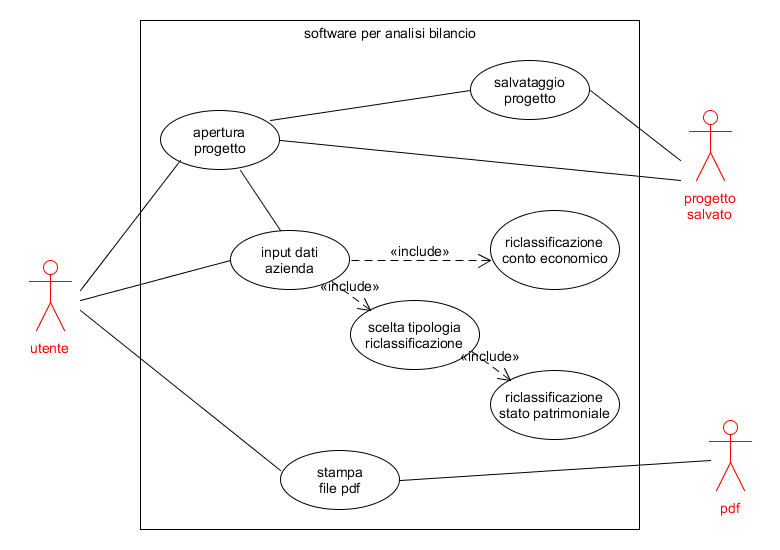
\includegraphics[scale=0.5]{use-case-diagram.png}
    \caption{UML Use Case Diagram}
    \label{fig:UseCase1}
\end{figure}

Nel diagramma in figura  ~\ref{fig:UseCase1} abbiamo tre attori, l'utente che inserisce i dati dell'azienda, il file contenente il progetto salvato e il file pdf generato dal software.
I casi d'uso talvolta includono più passaggi al loro interno, in quei casi è indicata una freccia "include", come nel caso del "input dati azienda" che include "scelta tipologia riclassificazione" che a sua volta include "riclassificazione stato patrimoniale".

% 3.4

\newpage

\section{Activity diagram}

L'Activity Diagram è un diagramma che definisce le attività da svolgere per realizzare una data funzionalità ed è spesso utilizzato come modello complementare dello Use Case Diagram.

\begin{figure}[H]
    \centering
    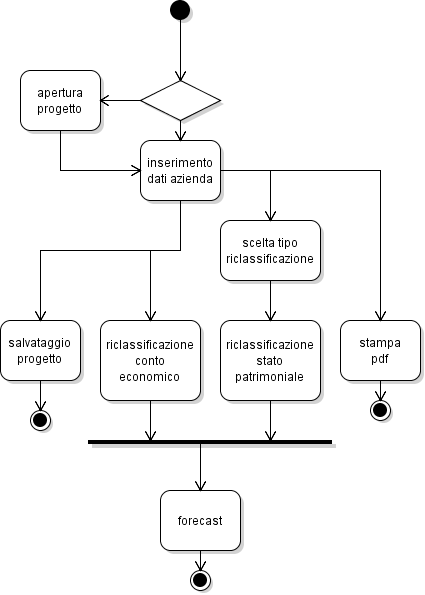
\includegraphics[scale=0.6]{activity-diagram.png}
    \caption{UML Activity Diagram}
    \label{fig:ActivityDiagram1}
\end{figure}

Nella figura ~\ref{fig:ActivityDiagram1} vediamo descritto il software come nello Use Case precedente, ma dal punto di vista delle attività da svolgere in sequenza per raggiungere un certo risultato.
Il diagramma si legge a partire dal pallino in alto, detto nodo iniziale, seguono le azioni indicate dai rettangoli.
I rombi indicano le decisioni, cioè le diverse direzioni che può prendere il flusso a seguito di certe condizioni o scelte, ad esempio all'avvio del software se si vuole aprire un progetto salvato precedentemente o inserire i dati per un nuovo progetto.
Un altro elemento dell'activity diagram è la "join", che indica che per passare all'azione successiva devono essere completate tutte le azioni in ingresso, come ad esempio per il calcolo del forecast, che avviene una volta inseriti i dati e quindi calcolate le riclassificazioni dello
stato patrimoniale e del conto economico.

% 3.5

\newpage

\section{Sequence diagram}

Il sequence diagram è uno strumento di modellazione visuale che mette in evidenza come i vari componenti di un sistema interagiscono tra di loro in relazione al tempo.

\begin{figure}[H]
    \centering
    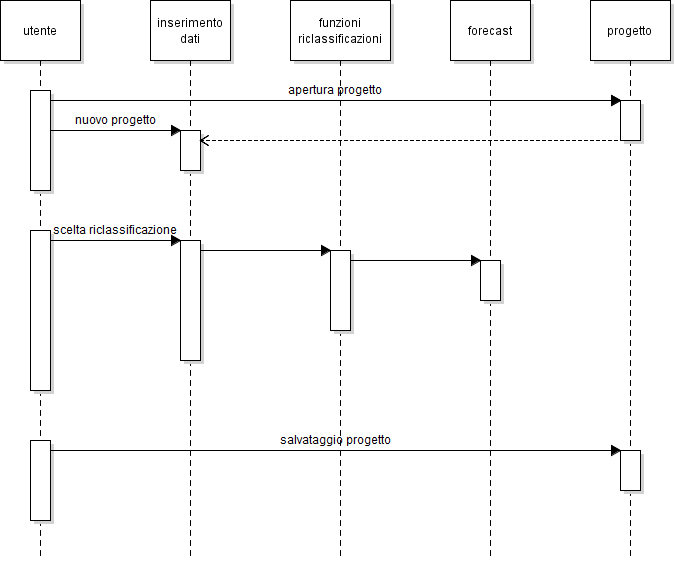
\includegraphics[scale=0.6]{sequence-diagram.png}
    \caption{UML Sequence Diagram}
    \label{fig:SequenceDiagram}
\end{figure}

Nella figura ~\ref{fig:SequenceDiagram} vediamo descritto il flusso iniziale del software che inizia con la scelta da parte dell'utente di creazione di un nuovo progetto o di aprire un progetto salvato precedentemente e termina con il salvataggio dello stesso dopo aver calcolato tutte le riclassificazioni.
I componenti del diagramma sono l'utente, la form che permette l'input dei dati, le funzioni per le riclassificazioni, la funzione del forecast e il progetto salvato esternamente.
Nella fase di inserimento dei dati da parte dell'utente, il sistema calcola le varie riclassificazioni, tendendo conto della scelta dell'utente della tipologia scelta per lo Stato Patrimoniale, e mette tutto a disposizione per il salvataggio dei dati e per la stampa del pdf.
    
    % White page
    \clearpage\null\newpage
    
    % Sviluppo
    % 4

\chapter{Sviluppo}

Quando si vuole sviluppare un’applicazione desktop la prima cosa a cui si pensa è per quale sistema operativo svilupparla, quale linguaggio usare ed opzionalmente a quale base dati si ha bisogno di connettersi.
In questo caso la scelta è caduta su Electron, un framework Open Source sviluppato dal team di GitHub che permette lo sviluppo di app cross platform utilizzando il medesimo approccio di Apache Cordova, ovvero attraverso JavaScript, HTML, e CSS.
Si tratta di un modulo Npm, quindi eredita tutte le API e le funzionalità di Node.js.
\\
Electron, è ormai considerato un package stabile, arrivato alla versione 1.3.9, dispone di molti plugin già pronti all’uso e realizzati specificamente per la piattaforma. Tuttavia, il vero potenziale di Electron è dato dal fatto che si può costruire una desktop app utilizzando qualsiasi libreria scritta in Node.js, rendendolo di fatto uno strumento molto potente anche per interagire con il sistema operativo.
\\
Nello specifico dello sviluppo del sofware, si possono distinguere tre specifiche aree:
\begin{itemize}
	\item Back-End, comprende tutto ciò che riguarda lo sviluppo della logica del software, ovvero cosa fare con i dati, come trattare quelli ricevuti, cosa restituire all'utente.
	\item Front-End, comprende tutto ciò che riguarda l'interfaccia utente, quindi come presentare i dati passati dal Back-End, la grafica, il template, il typewriting, l’accessibilità e l’usabilità.
	\item Packaging dell'App, la creazione del prodotto finale, ovvero il software in versione eseguibile per tutte le tipologie di piattaforme di elaborazione.
\end{itemize}


% 4.1

\section{Sviluppo del Back-End}

Nella struttura di un app basata su Electron, bisogna discutere di due tipi di processo esistenti:
\begin{itemize}
	\item  il processo chiamato \textbf{main} che esegue lo script indicato nel file package.json è il processo principale. Lo script che viene eseguito nel processo principale può visualizzare una \Gls{GUI} tramite la creazione di pagine web. Una applicazione Electron ha sempre un 		processo principale, ma mai più di uno. Il processo principale crea pagine web mediante la creazione di istanze di BrowserWindow, dove viene eseguita la pagina web nel proprio processo di rendering. Quando viene eliminata un'istanza di BrowserWindow, il processo di 		rendering corrispondente viene anch'esso terminato. Il processo principale gestisce tutte le pagine web e il corrispondente processo di rendering.
	\item il processo di \textbf{rendering}, invece è il processo che gestisce ogni pagina web, visualizzata tramite Chromium con la sua architettura multi-processo, tale processo è isolato e può occuparsi solo delle pagine web in esecuzione in esso.
	Pertanto nelle pagine web chiamare le API dell'interfaccia grafica nativa non è consentito perché la gestione delle risorse di sistema nelle pagine web è molto pericolosa ed è facile perdere risorse. Se si desidera eseguire operazioni di \Gls{GUI} in una pagina web, il processo di 		rendering della pagina web deve comunicare con il processo principale per richiedere che il processo principale esegua tali operazioni.
\end{itemize}

\begin{figure}[H]
    \centering
    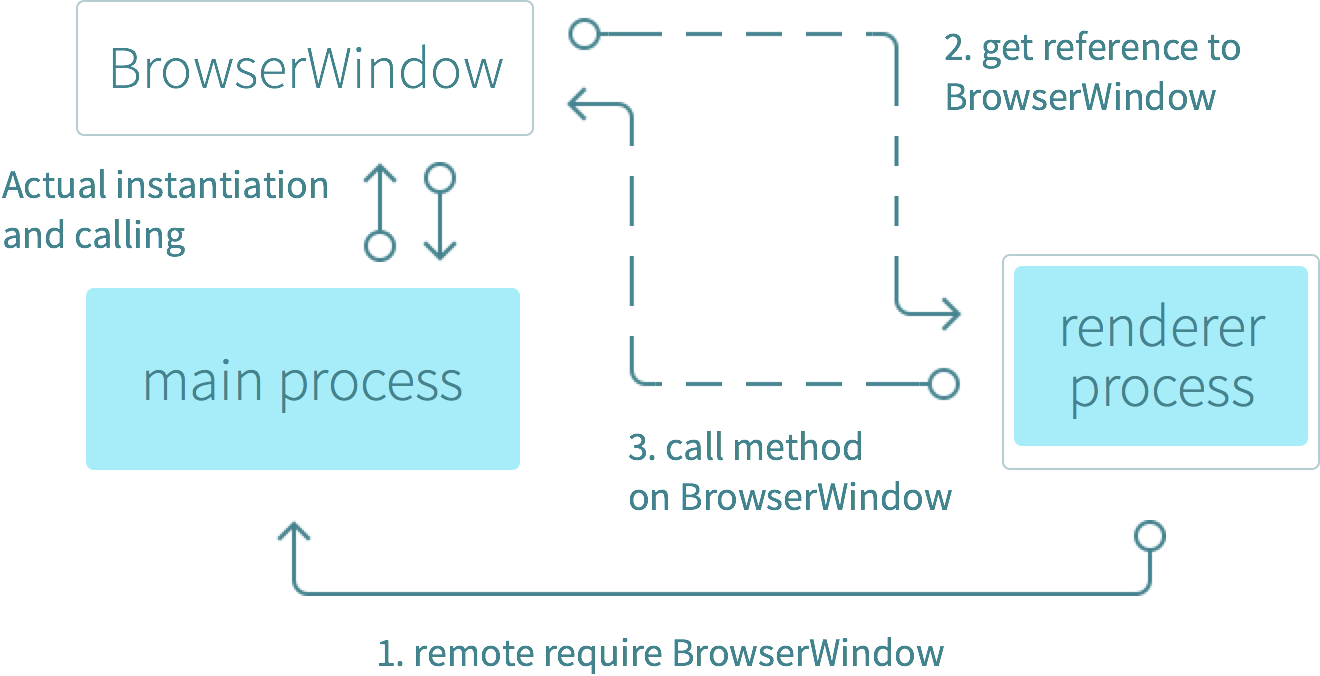
\includegraphics[scale=0.25]{electron-architecture.png}
    \caption{Electron - Architettura di un app}
    \label{fig:ElectronArch}
\end{figure}

% 4.1.1

\subsection{Utilizzo delle API Electron}


% 4.1.2

\subsection{Utilizzo API Node.js}


% 4.1.3

\subsection {Calcolo riclassificazioni e forecast}

% 4.1.4

\subsection {Apertura e salvataggio progetto}

% 4.1.5

\subsection {Creazione pdf}


% 4.2

\newpage

\section{Sviluppo del Front-End}

Per lo sviluppo di un interfaccia utente efficace si deve tener conto di due aspetti oltre a quello tecnico, che sono:
\begin{itemize}
\item Accessibilità
\item Usabilità
\end{itemize}

L'\textbf{usabilità} è un approccio alla progettazione volto a rendere l'interazione tra il prodotto e l'utente migliore sotto i seguenti aspetti:
\begin{itemize}
    \item Efficacia, cioè permettere agli utenti di raggiungere i loro obiettivi in maniera precisa e completa;
    \item Efficienza, cioè l'ottimizzazione delle risorse impiegate;
    \item Soddisfazione, come libertà dal disagio e attitudine positiva con cui gli utenti raggiungono specifici obiettivi attraverso l’uso del prodotto.
\end{itemize}
Nel web, l'usabilità si pone i seguenti obiettivi:
\begin{itemize}
    \item Presentare l'informazione all'utente in modo chiaro e conciso, evitando termini tecnici o specialistici;
    \item Semplificare la struttura del compito;
    \item Offrire all'utente le scelte corrette, in una maniera che risulti ovvia;
    \item Organizzare ogni pagina in modo che l'utente riconosca la posizione e le azioni da compiere;
    \item Eliminare ogni ambiguità relativa alle conseguenze di un'azione (es. fare clic su cancella/rimuovi/compra);
    \item Mettere la cosa più importante nella posizione giusta della pagina web o dell'applicazione web;
    \item Fare in modo che l'utente abbia un rapido feedback ad ogni azione compiuta, ad esempio la comparsa di un messaggio di successo o errore all'invio di dati con una form;
    \item Rendere la grafica accattivante ed interessante dal punto di vista visivo attraverso l'uso di diagrammi, tabelle, sezioni informative e coordinando bene i colori;
    \item Ridurre gli sforzi cognitivi dell'utente.
\end{itemize}
In generale cercare di rendere il sistema il più semplice possibile da usare, in modo da ridurre al minimo gli sforzi sull'utilizzo del mezzo.

L'\textbf{accessibilità} è un aspetto di fontamentale importanza, specialmente per un gestionale web di una ; il suo scopo è garantire l'accesso alle risorse (prodotti e servizi) da parte di chiunque, siano essi soggetti con disabilità, con scarse competenze informatiche o con dispositivi diversi.
I criteri dell'accessibilità sono quelli delle linee guida del  che attraverso una sua sezione denominata  ha definito i linguaggi e le procedure standard per rendere il Web uno strumento realmente democratico e universale.
Queste direttive sono state percepite in Italia con la Legge "Stanca" (Legge 4/2004) che sancisce obblighi e sanzioni per la  e le aziende appaltate.
In generale i requisiti di accessibilità contenuti nella Legge Stanca e successive modificazioni, contenuti anche in un documento online sul sito del governo , sono i seguenti:
\begin{itemize}
    \item Alternative testuali, obbligatorie per tutte i contenuti non testuali (come immagini, filmati e audio);
    \item Adattabilità, cioè prevedere che i contenuti si adattino a diversi layout in base alla grandezza e al formato dello schermo utente (responsive web design);
    \item Distinguibile, rendere più semplice agli utenti la visione e l'ascolto dei contenuti, separando i contenuti in primo piano dallo sfondo;
    \item Accessibile da tastiera, cioè garantire una buona navigabilità prevedendo un percorso di TAB;
    \item Colori, il contrasto tra le scritte e lo sfondo deve essere chiaro, ma non si devono usare colori discordanti tra loro o lampeggianti che possano causare crisi epilettiche;
    \item Navigabile, fornire una struttura del sito chiara, dove l'utente possa orientarsi e raggiungire qualsiasi sezione attraverso links;
    \item Assistenza per l'inserimento, fornire gli aiuti e le spiegazioni necessarie affinché l'utente sia in grado di compilare correttamente le form del sito;
    \item Compatibilità, il sito deve essere accessibile da tutte le piattaforme e deve utilizzare tecnologie standard.
\end{itemize}

% 4.2.1

\subsection{Tecnologie usate nello sviluppo del front-end}

Mentre per lo sviluppo del back-end abbiamo a disposizione una gran quantità di tecnologie concorrenti per svolgere lo stesso compito, per il front-end le tecnologie di base sono sempre le stesse: \Gls{html}, \Gls{css} e JavaScript.

\textbf{\Gls{html}} è un linguaggio di markup per le pagine web i cui standard sono definiti dal e serve per descrivere il contenuto di una pagina web, sia testuale che multimediale, attraverso dei tag.
Sebbene il linguaggio sia in grado di definire anche regole di formattazione come la centratura del testo o la dimensione dei caratteri, il suo scopo primario è quello di descrivere i contenuti e il loro significato semantico, attraverso l'uso dei tag appropriati (ad esempio \textless p\textgreater  per i paragrafi, \textless h1\textgreater  per un titolo di primo livello, \textless  address\textgreater  per informazioni relative ad un indirizzo, etc.).
Attualmente la versione più recente delle specifiche è chiamata HTML 5 e comporta rispetto alle precedenti versioni l'aggiunta di alcuni tag per gli elementi multimediali, il miglioramento i controlli di input per le form, il controllo della geolocalizzazione e l'intruduzione dello Web Storage come alternativa ai cookies.

\textbf{\Gls{css}}  è il linguaggio usato per definire il layout (impaginazione), la formattazione del testo e l'aspetto grafico in generale; può essere definito sia all'interno della pagina \Gls{html} che all'esterno come file a sé stante, che è generalamente la scelta migliore.
Nel nostro caso sono state usate alcune delle proprietà più recenti del linguaggio come la box-shadow o la border-radius appartenenti alle specifiche CSS 3.
Per mantenere la compatibilità tra i differenti browser (e nei limiti del possibile anche con le versioni più vecchie degli stessi) sono state applicate ad ogni proprietà CSS 3 delle tecniche di cross-browsing, cioè la riscrittura della stessa proprietà in modi differenti, vedi figure ~\ref{fig:Css3Shadow} e ~\ref{fig:Css3Radius}.

\begin{figure}[H]
    \centering
    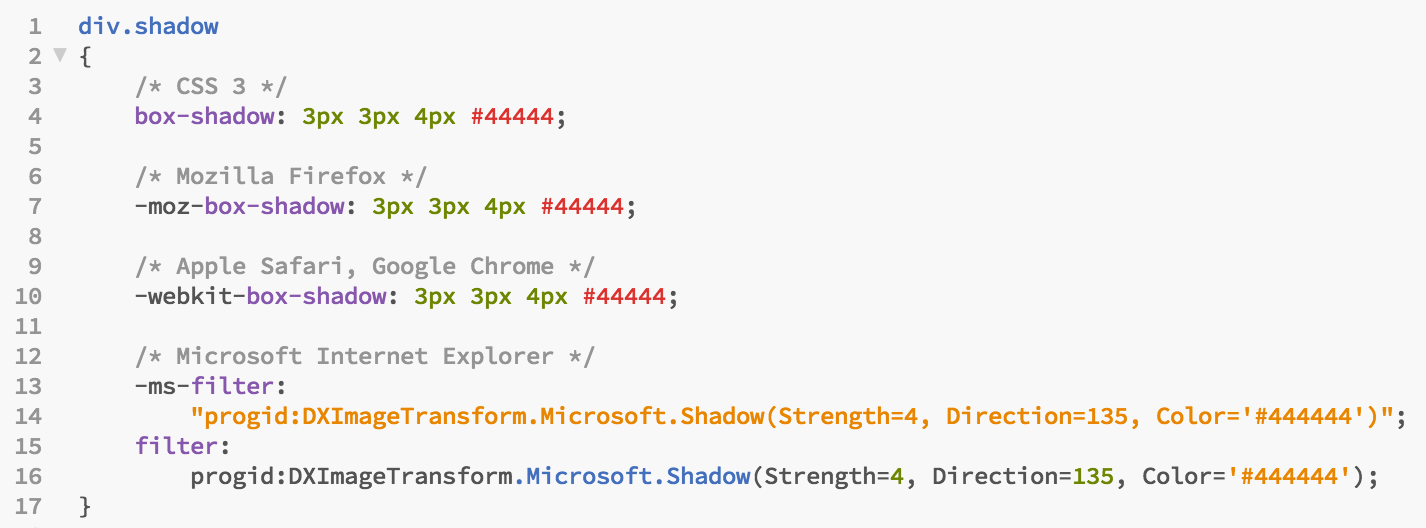
\includegraphics[scale=0.5]{css3-1.png}
    \caption{CSS 3 text-shadow cross-browser}
    \label{fig:Css3Shadow}
\end{figure}

\begin{figure}[H]
    \centering
    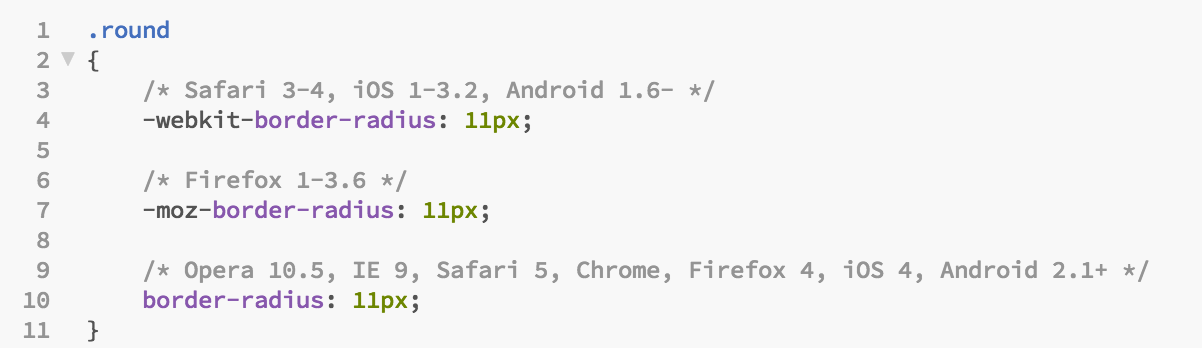
\includegraphics[scale=0.5]{css3-2.png}
    \caption{CSS 3 border-radius cross-browser}
    \label{fig:Css3Radius}
\end{figure}

\textbf{JavaScript} è un linguaggio di scripting adatto per creare effetti dinamici interattivi basati su eventi, come il click di un bottone, la selezione di una voce da una tendina, la pressione di un tasto o il caricamento di una pagina.
Anche se con il javascript è possibile creare applicazioni vere e proprie si deve sempre tener conto che è un linguaggio accessorio, ovvero c'è la possibilità per l'utente di disabilitarlo, specialmente nel caso si abbia delle disabilità o dei problemi di visualizzazione.
Pertanto nessuna funzionalità deve contare unicamente su javascript per funzionare, ma il suo uso è comunque consigliato per aumentare l'esperienza utente (quegli obiettivi dell'usabilità esposti sopra) ad esempio prevedendo dei messaggi di errore nel caso si inseriscano dei valori errati nei campi, o un calendario all'immissione di un campo data, o anche per sostituire delle proprietà del CSS 3 nel caso il browser dell'utente non la supporti (i cosiddetti polyfill).

\textbf{jQuery}  è una libreria Javascript molto diffusa il cui scopo è semplificare la selezione, la gestione e la manipolazione degli eventi, mantenendo però anche la possibilità di utilizzare il linguaggio nella vecchia maniera.
L'uso di jQuery non aggiunge quindi nessuna funzionalità, rende solamente più semplice l'utilizzo del linguaggio e quindi più elevata la produttività del programmatore, non a caso il suo motto è "Write less, do more", anch'essa è stata inclusa nella nostra applicazione web e gli script personalizzati fanno tutti riferimento alla sua sintassi.

 è un'altra tecnologia molto importante per migliorare l'esperienza utente, perché permette di aggiornare il contenuto di una pagina dinamicamente senza effettuare il "refresh" e quindi caricando solo le informazioni necessarie, anziché tutta la pagina.
Si tratta, più che di un nuovo linguaggio, di un insieme di tecniche che fanno uso delle tecnologie sopra descritte, quindi JavaScript per inviare le richieste asincrone e XML o JSON per ricevere le risposte dal server sottoforma di oggetti.
Questa tecnica è stata utilizzata nella nostra applicazione web nella fase di autenticazione post-Cohesion, dove viene richiesto all'utente di scegliere un ruolo da una tendina e automaticamente sulla base di questa scelta viene popolata la tendina delle riferite a quel ruolo.
Un altro utilizzo è nella pagina di inserimento di un nuovo utente, dove a seguito della digitazione di almeno 3 caratteri in una casella di testo, compare un menù di autocomplete che suggerisce i possibili nomi degli utenti cercati.

\textbf{Razor}  infine, è un linguaggio di programmazione lato server, specifico del framework ASP.NET MVC, ma è stato incluso in questa sezione perché serve a descrivere, insieme all'HTML, il contenuto di una View.
Una View che contiene codice Razor sarà un file di tipo .cshtml (nel caso il linguaggio lato server utilizzato sia il C).
Questo linguaggio può utilizzare molte delle classi del framework, semplicemente includendo il namespace nella pagina, ma il suo scopo principale è quello di posizionare gli elementi del Model nella View, passati dal Controller, eventualmente anche iterando una Collection affinché venga stampata a schermo una serie di elementi per ogni elemento della Collection, come in Figura ~\ref{fig:Razor}.

\begin{figure}[H]
    \centering
    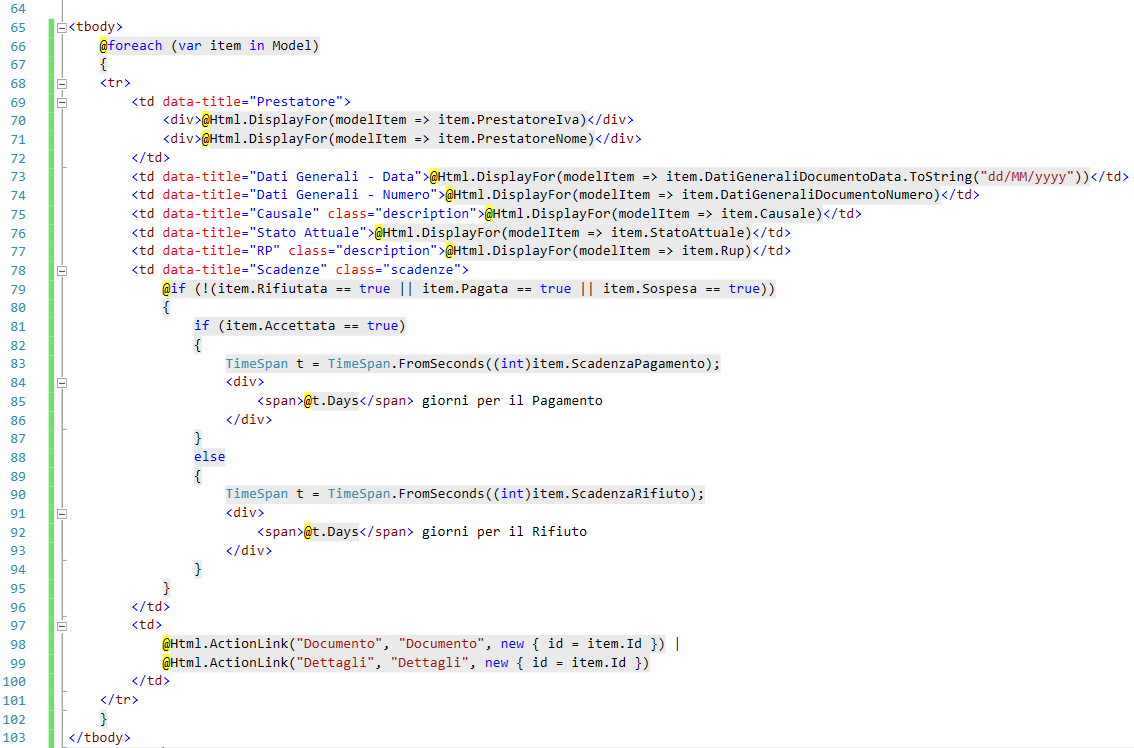
\includegraphics[scale=0.5]{razor-1.png}
    \caption{Esempio di codice Razor per la stampa degli elementi di una collection come righe di una tabella HTML}
    \label{fig:Razor}
\end{figure}


% 4.3

\newpage

\section{Packaging dell'applicazione}

Per lo sviluppo di un interfaccia utente efficace si deve tener conto di due aspetti oltre a quello tecnico, che sono:
\begin{itemize}
\item Accessibilità
\item Usabilità
\end{itemize}

L'\textbf{usabilità} è un approccio alla progettazione volto a rendere l'interazione tra il prodotto e l'utente migliore sotto i seguenti aspetti:
\begin{itemize}
    \item Efficacia, cioè permettere agli utenti di raggiungere i loro obiettivi in maniera precisa e completa;
    \item Efficienza, cioè l'ottimizzazione delle risorse impiegate;
    \item Soddisfazione, come libertà dal disagio e attitudine positiva con cui gli utenti raggiungono specifici obiettivi attraverso l’uso del prodotto.
\end{itemize}
Nel web, l'usabilità si pone i seguenti obiettivi:
\begin{itemize}
    \item Presentare l'informazione all'utente in modo chiaro e conciso, evitando termini tecnici o specialistici;
    \item Semplificare la struttura del compito;
    \item Offrire all'utente le scelte corrette, in una maniera che risulti ovvia;
    \item Organizzare ogni pagina in modo che l'utente riconosca la posizione e le azioni da compiere;
    \item Eliminare ogni ambiguità relativa alle conseguenze di un'azione (es. fare clic su cancella/rimuovi/compra);
    \item Mettere la cosa più importante nella posizione giusta della pagina web o dell'applicazione web;
    \item Fare in modo che l'utente abbia un rapido feedback ad ogni azione compiuta, ad esempio la comparsa di un messaggio di successo o errore all'invio di dati con una form;
    \item Rendere la grafica accattivante ed interessante dal punto di vista visivo attraverso l'uso di diagrammi, tabelle, sezioni informative e coordinando bene i colori;
    \item Ridurre gli sforzi cognitivi dell'utente.
\end{itemize}
In generale cercare di rendere il sistema il più semplice possibile da usare, in modo da ridurre al minimo gli sforzi sull'utilizzo del mezzo.

L'\textbf{accessibilità} è un aspetto di fontamentale importanza, specialmente per un gestionale web di una ; il suo scopo è garantire l'accesso alle risorse (prodotti e servizi) da parte di chiunque, siano essi soggetti con disabilità, con scarse competenze informatiche o con dispositivi diversi.
I criteri dell'accessibilità sono quelli delle linee guida dche attraverso una sua sezione denominata ha definito i linguaggi e le procedure standard per rendere il Web uno strumento realmente democratico e universale.
Queste direttive sono state percepite in Italia con la Legge "Stanca" (Legge 4/2004) che sancisce obblighi e sanzioni per e le aziende appaltate.
In generale i requisiti di accessibilità contenuti nella Legge Stanca e successive modificazioni, contenuti anche in un documento online sul sito del governsono i seguenti:
\begin{itemize}
    \item Alternative testuali, obbligatorie per tutte i contenuti non testuali (come immagini, filmati e audio);
    \item Adattabilità, cioè prevedere che i contenuti si adattino a diversi layout in base alla grandezza e al formato dello schermo utente (responsive web design);
    \item Distinguibile, rendere più semplice agli utenti la visione e l'ascolto dei contenuti, separando i contenuti in primo piano dallo sfondo;
    \item Accessibile da tastiera, cioè garantire una buona navigabilità prevedendo un percorso di TAB;
    \item Colori, il contrasto tra le scritte e lo sfondo deve essere chiaro, ma non si devono usare colori discordanti tra loro o lampeggianti che possano causare crisi epilettiche;
    \item Navigabile, fornire una struttura del sito chiara, dove l'utente possa orientarsi e raggiungire qualsiasi sezione attraverso links;
    \item Assistenza per l'inserimento, fornire gli aiuti e le spiegazioni necessarie affinché l'utente sia in grado di compilare correttamente le form del sito;
    \item Compatibilità, il sito deve essere accessibile da tutte le piattaforme e deve utilizzare tecnologie standard.
\end{itemize}

    
    % Lavori simili
    \chapter{Possibili sviluppi futuri}

Ogni regione è stata chiamata per legge a sviluppare il proprio sistema di fatturazione e, eventualmente, a porsi come nodo locale di interscambio per le fatture degli enti locali.
In Regione Lazio il sistema \textbf{HUB} \cite{hub} svolge appunto questo ruolo, esso prevede un sito per l'adesione al sistema da parte delle \Gls{ppaa} e dei privati a tre tipi di servizio: fattura attiva, fattura passiva, conservazione.
La Regione Emilia-Romagna predispone anch'essa un sistema di interscambio regionale chiamato \textbf{NoTI-ER} \cite{notier}, il quale una volta ricevuta la fattura dallo \Gls{sdi} prima la converte nel formato europeo PEPPOL \cite{peppol}, poi la invia al software \textbf{SICIPA-ER} (l'equivalente del nostro Fatto) e al sistema di conservazione Par-ER.
Troviamo un sistema di interscambio anche per la Regione Toscana, chiamato \textbf{fERT}, che oltre alla comunicazione tra \Gls{sdi} e Ente, si occupa anche della comunicazione con la \Gls{pcc}.
In Regione Marche il ruolo di intermediario svolto da \Gls{imm} \cite{intermedia} è quello di mettere in comunicazione lo \Gls{sdi}, con Fatto e Fatto con il sistema di protocollo, quindi presiede a tutto il processo di fatturazione fino al momento dell'accettazione/rifiuto.
Successivamente le comunicazioni con la \Gls{pcc} passano per il software della contabilità Siagi, il quale prima di inviare i dati relativi ai pagamenti, preleva le informazioni necessarie (associazioni tra fatture e decreti, tempi di accettazione e contabilizzazione, etc) da Fatto.

%\chapter{Deploy e manutenzione}

%\section{Le fasi di produzione}

%\section{Compilazione}

%\section{Pubblicazione}

%\section{Cattura e gestione degli errori}

    
    % White page
    \clearpage\null\newpage
    
    % Conclusione
    \chapter*{Conclusione}
\addcontentsline{toc}{chapter}{Conclusione}
\markboth{CONCLUSION}{}

La mia collaborazione alla realizzazione di questo progetto mi ha permesso di valutare in un contesto concreto l'efficacia sia delle metodologie di analisi e progettazione, sia delle tecnologie di sviluppo utilizzate.
Essendo stato partecipe inoltre ad alcuni processi decisionali nel ruolo di referente tecnico, ho potuto confermare l'importanza di una buona scrittura dei requisiti funzionali e non, accompagnata da una gestione delle attività e delle scadenze.

Dal punto di vista del personale amministrativo non ci sono state difficoltà nell'apprendere l'utilizzo del software, anche grazie agli accorgimenti presi per il front-end e alla continua disponibilità, mia e dei miei referenti.
In ogni caso alcune problematiche di dominio sono venute fuori solo successivamente al rilascio della prima versione del software, ciò ha comportato un continuo lavoro di rianalisi e riadattamento che ha interessato tutte le parti responsabili dei software coinvolti nel processo di fatturazione.

Parlando di vantaggi al cittadino, da un lato si sono ottenuti dei tempi certi per quanto riguarda l'accettazione e il rifiuto (garantiti dalla spietatezza dei contatori informatici) e si è indirettamente dato uno standard ai vari software proprietari e non per la gestione delle fatture.
Da un altro lato però sono aumentati gli oneri per i fornitori, perché anche ammettendo che si riesca a realizzare autonomamente l'xml della fattura da inviare o che il vecchio software di fatturazione in proprio possesso sia stato aggiornato senza ulteriori spese, si deve far fronte alle spese per la conservazione digitale, ovvero alle spese per un software di conservazione aderente agli standard e alle marche temporali digitali.

Tutti questi problemi spero si risolvano nel futuro, scegliendo magari di gestire la conservazione direttamente lato \Gls{sdi}, con un maggiore sforzo implementativo da parte del Ministero.

Complessivamente mi ritengo soddisfatto di quanto fatto finora, ma sono consapevole che la realizzazione del progetto non è che un passo verso una complessiva digitalizzazione e sostanziale modifica del funzionamento della \Gls{pa}.

I futuri sviluppi che interesseranno il sistema di fatturazione saranno legati al prossimo rilascio da parte della \Gls{pcc} dei web service per lo scambio delle informazioni relative ai pagamenti effettuati.
Non è esclusa tuttavia anche una possibile adozione degli standard PEPPOL, relativi al processo di fatturazione o anche una parziale ridefinizione di alcuni processi amministrativi digitali.
        
    \chapter*{Dediche}

    \appendix
        
    % Glossario
    \printglossary[type=\acronymtype]
    \printglossary
     
    % Bibliografia
    \printbibheading
    \printbibliography[type=book,heading=subbibliography,title={Libri}]
    \printbibliography[type=online,heading=subbibliography,title={Sitografia}]

\end{document}